%%%%%%%%%%%%%%%%%%%%%%%%%%%%%%%%%%%%%%%%%%%%%%%%%%%%%%%%%%%%%%%%%%%%%%%%%%%%%%%%%%%%%%%%%%%%%%%%%%%
%%%%%%%%%%%%%%%%%%%%%%%%%%%%%%%%%%%%%%%%%%%%%%%%%%%%%%%%%%%%%%%%%%%%%%%%%%%%%%%%%%%%%%%%%%%%%%%%%%%
%%%%%%%%%%%%%%%%%%%%%%%%%%%%%%%%%%%%%%%%%%%%%%%%%%%%%%%%%%%%%%%%%%%%%%%%%%%%%%%%%%%%%%%%%%%%%%%%%%%
\documentclass[12pt,dvipdfmx]{beamer}
%%%%%%%%%%%%%%%%%%%%%%%%%%%%%%%%%%%%%%%%%%%%%%%%%%%%%%%%%%%%%%%%%%%%%%%%%%%%%%%%%%%%%%%%%%%%%%%%%%%%%%
% pdfの栞・プロパティの字化けを防ぐ
\usepackage{atbegshi}
%\AtBeginShipoutFirst{\special{pdf:tounicode 90ms-RKSJ-UCS2}} %Windows
\AtBeginShipoutFirst{\special{pdf:tounicode EUC-UCS2}} %Linux, Mac
\usepackage{hyperref}
%%%%%%%%%%%%%%%%%%%%%%%%%%%%%%%%%%%%%%%%%%%%%%%%%%%%%%%%%%%%%%%%%%%%%%%%%%%%%%%%%%%%%%%%%%%%%%%%%%%%%%
%%%
%%% テーマの指定、省略時は default になる
%%%

 % フレームの指定、省略可
%%%%%%%%%%%%%%%%%%%%%%%%%%%% THEME
  %\usetheme{AnnArbor}
  %\usetheme{Antibes}
  %\usetheme{Bergen}
  %\usetheme{Berkeley}
  %\usetheme{Berlin}
  \usetheme{Boadilla}
  %\usetheme{boxes}
  %\usetheme{CambridgeUS}
  %\usetheme{Copenhagen}
  %\usetheme{Darmstadt}
  %\usetheme{default}
  %\usetheme{Dresden}
  %\usetheme{Frankfurt}
  %\usetheme{Goettingen}
  %\usetheme{Hannover}
  %\usetheme{Ilmenau}
  %\usetheme{JuanLesPins}
  %\usetheme{Luebeck}
  %\usetheme{Madrid}
  %\usetheme{Malmoe}
  %\usetheme{Marburg}
  %\usetheme{Montpellier}
  %\usetheme{PaloAlto}
  %\usetheme{Pittsburgh}
  %\usetheme{Rochester}
  %\usetheme{Singapore}
  %\usetheme{Szeged}
  %\usetheme{Warsaw}
% 省略可
%%%%%%%%%%%%%%%%%%%%%%%%%%%% COLOR THEME
  %\usecolortheme{albatross}
  %\usecolortheme{beetle}
  %\usecolortheme{crane}
  %\usecolortheme{default}
  %\usecolortheme{dolphin}
  %\usecolortheme{dove}
  %\usecolortheme{fly}
  %\usecolortheme{lily}
  %\usecolortheme{orchid}
  %\usecolortheme{rose}
  %\usecolortheme{seagull}
  %\usecolortheme{seahorse}
  %\usecolortheme{sidebartab}
  %\usecolortheme{structure}
  %\usecolortheme{whale}

% ヘッダ、フッタ、フレーム等を指定、省略可
  %%%%%%%%%%%%%%%%%%%%%%%%%%%% OUTER THEME
  %\useoutertheme{default}
  %\useoutertheme{infolines}
  %\useoutertheme{miniframes}
  %\useoutertheme{shadow}
  %\useoutertheme{sidebar}
  %\useoutertheme{smoothbars}
  %\useoutertheme{smoothtree}
  %\useoutertheme{split}
  %\useoutertheme{tree}

% タイトル、section, itemize/enumerate 環境、
% theorem 環境、図, 参考文献などのスタイルを指定、
% 省略可
  %%%%%%%%%%%%%%%%%%%%%%%%%%%% INNER THEME
  %\useinnertheme{circles}
  %\useinnertheme{default}
  %\useinnertheme{inmargin}
  \useinnertheme{rectangles}
  %\useinnertheme{rounded}


%\usefonttheme{}	% 省略可
%\logo{}		% 省略可

%%%%%%%%%%%%%%%%%%%%%%%%%%%%%%%%%%%%%%%%%%%%%%%%%%%%%%%%%%%%%%%%%%%%%%%%%%%%%%%%%%%%%%%%%%%%%%%%%%%
%%%%%%%%%%%%%%%%%%%%%%%%%%%%%%%%%%%%%%%%%%%%%%%%%%%%%%%%%%%%%%%%%%%%%%%%%%%%%%%%%%%%%%%%%%%%%%%%%%%
%%%%%%%%%%%%%%%%%%%%%%%%%%%%%%%%%%%%%%%%%%%%%%%%%%%%%%%%%%%%%%%%%%%%%%%%%%%%%%%%%%%%%%%%%%%%%%%%%%%
% navi. symbolsは目立たないが,dvipdfmxを使うと機能しないので非表示に
\setbeamertemplate{navigation symbols}{}

% 各種パッケージ
\usepackage{graphicx}
%\usepackage{url,cite}
\usepackage{amsmath}
\usepackage{amsthm} \theoremstyle{definition} %theorem環境が斜体になるので注意
\usepackage{amssymb} % AMS-TeX
\usepackage{setspace}

% \AtBeginSection[] % Do nothing for \section*
% { \begin{frame}<beamer> \frametitle{}
%    \tableofcontents[currentsection,subsectionstyle=hide]
%  \end{frame} } 

%appendixをページカウントしない
\newcommand{\backupbegin}{
   \newcounter{framenumberappendix}
   \setcounter{framenumberappendix}{\value{framenumber}}
}
\newcommand{\backupend}{
   \addtocounter{framenumberappendix}{-\value{framenumber}}
   \addtocounter{framenumber}{\value{framenumberappendix}} 
}

%%%%%%%%%%%%%%%%%%%%%%%%%%%%%%%%%%%%%%%%%%%%%%%%%%%%%%%%%%%%%%%%%%%%%%%%%%%%%%%%%%%%%%%%%%%%%%%%%%%%%%
% 本文・数式フォント
%\usepackage{palatino,mathpazo}
%\usepackage{times,mathptmx}
\usepackage[varg]{txfonts}
%\usepackage[varg]{pxfonts}

% \mathcal(\cal)の扱い
%\DeclareMathAlphabet{\mathcal}{OMS}{cmsy}{m}{n} %computer modern
%\DeclareMathAlphabet{\mathcal}{OMS}{txsy}{m}{n} %txfont
%\usepackage[psamsfonts]{eucal} % euler

% mathptmx時に数式モードのvをtxfontから借りる
% \DeclareSymbolFont{lettersA}{U}{txmia}{m}{it}
% \SetSymbolFont{lettersA}{bold}{U}{txmia}{bx}{it}
% \DeclareFontSubstitution{U}{txmia}{m}{it}
% \DeclareMathSymbol{v}{\mathalpha}{lettersA}{"33} %"


%上線 widebar, Widebar
\usepackage{accents}
\makeatletter
\def\widebar{\accentset{{\cc@style\underline{\mskip11mu}}}}
\makeatother


%%%%%%%%%%%%%%%%%%%%%%%%%%%%%%%%%%%%%%%%%%%%%%%%%%%%%%%%%%%%%%%%%%%%%%%%%%%%%%%%%%%%%%%%%%%%%%%%%%%%%%

% 定理環境
% \newtheorem{theorem}{Theorem}
% \newtheorem{lemma}[theorem]{Lemma}
% \newtheorem{corollary}[theorem]{Corollary}
% \newtheorem{definition}[theorem]{Definition}
% \newtheorem{example}[theorem]{Example}
\newtheorem{proposition}{Proposition}
\newtheorem{remark}{Remark}

%%%%%%%%%%%%%%%%%%%%%%%%%%%%%%%%%%%%%%%%%%%%%%%%%%%%%%%%%%%%%%%%%%%%%%%%%%%%%%%%%%%%%%%%%%%%%%%%%%%%%%
% 各種コマンド定義等
\def\Fig#1{Fig.\@\ref{#1}}
\def\Table#1{Table~\ref{#1}}
\def\Eq#1{Eq.\@(\ref{#1})}
\def\Eqs#1{Eqs.\@(\ref{#1})}
\def\Thm#1{Theorem~\ref{#1}}
\def\Lma#1{Lemma~\ref{#1}}
\def\Sect#1{Section~\ref{#1}}
\def\Rmk#1{Remark~\ref{#1}}
\def\Prop#1{Proposition~\ref{#1}}
\def\Coro#1{Corollary~\ref{#1}}
\def\Def#1{Definition~\@\ref{#1}}
\def\Prob#1{Problem~\@\ref{#1}}
\def\ie{{i.\@e.\@,~}}
\def\eg{{e.\@g.\@,~}}
\def\etal{{et al.}}

% 数式環境用
\def\rank{\mathsf{rank}\, }
\def\dim{\mathsf{dim}\, }
\def\rspace{\mathsf{span}}
\def\supp{\mathsf{supp}}
%\def\vec#1{\mathbf{#1}}
\def\F{\mathbb{F}}
\def\wt{\mathsf{wt}}
\def\c{\mathcal{C}}
\def\dc{\mathcal{C}^{\perp}}
\def\d{\mathcal{D}}
\def\dd{\mathcal{D}^{\perp}}
\def\g{\mathcal{G}}
\def\dg{\mathcal{G}^{\perp}}
\def\p{\mathcal{P}}
% \def\rspace{\mathsf{span}}
\def\supp{\mathsf{supp}}
\def\ker{\mathsf{Ker\ }}

%\def\bari#1{\{\widebar{#1}\}}
\def\bari#1{\,\overline{{\!\{#1\}\!}}\,}
%\def\bari#1{\bar{\{#1\}}}
\def\vecxi{Z_{\bari{i}}}
%\def\vecsxi{\vec{z}_i}
\def\tvector{X}
\def\tpackets{X_1,\dots,X_n}
\def\mvector{S}
\def\mpackets{S_1,\dots,S_l}
\def\rvector{Y}
\def\wvector{W}
\def\cvector{C}
\def\cword{C_{1},\dots,C_{l+n}}
\def\pcword{C_{l+1},\dots,C_{l+n}}
\def\randvector{R}

\def\compmat{\Phi}

%%%%%%%%%%%%%%%%%%%%%%%%%%%%%%%%%%%%%%%%%%%%%%%%%%%%%%%%%%%%%%%%%%%%%%%%%%%%%%%%%%%%%%%%%%%%%%%%%%%
%%%%%%%%%%%%%%%%%%%%%%%%%%%%%%%%%%%%%%%%%%%%%%%%%%%%%%%%%%%%%%%%%%%%%%%%%%%%%%%%%%%%%%%%%%%%%%%%%%%
%%%%%%%%%%%%%%%%%%%%%%%%%%%%%%%%%%%%%%%%%%%%%%%%%%%%%%%%%%%%%%%%%%%%%%%%%%%%%%%%%%%%%%%%%%%%%%%%%%%
%%%
%%%  日本語フォントをゴシックに、数式フォントを太字に変更する
%%%
\renewcommand{\kanjifamilydefault}{\gtdefault}
\renewcommand{\familydefault}{\sfdefault}

\setbeamerfont{title}{size=\large,series=\bfseries}
\setbeamerfont{frametitle}{size=\large,series=\bfseries}
%\setbeamertemplate{frametitle}[default][center]
\usefonttheme{professionalfonts} 

%\mathversion{bold} %数式フォントを太字に

%\def\vec#1{\mbox{\boldmath $#1$}}


%\logo{\includegraphics[width=2cm]{titech_logo.eps}}

%\setbeamertemplate{caption}[numbered]
%%%
%%% 著者など
%%%
\title[E2E Security with JS 03]{JavaScriptによるEnd-to-Endセキュリティ}
\subtitle{第3回 公開鍵暗号はどうやって使えばいいのか? 編}
\author[Jun Kurihara]{栗原 淳}
\institute[]{}
\date[]{}

%%%%%%%%%%%%%%%%%%%%%%%%%%%%%%%%%%%%%%%%%%%%%%%%%%%%%%%%%%%%%%%%%%%%%%%%%%%%%%%%%%%%%%%%%%%%%%%%%%%
%%%%%%%%%%%%%%%%%%%%%%%%%%%%%%%%%%%%%%%%%%%%%%%%%%%%%%%%%%%%%%%%%%%%%%%%%%%%%%%%%%%%%%%%%%%%%%%%%%%
%%%%%%%%%%%%%%%%%%%%%%%%%%%%%%%%%%%%%%%%%%%%%%%%%%%%%%%%%%%%%%%%%%%%%%%%%%%%%%%%%%%%%%%%%%%%%%%%%%%
%%%%%%%%%%%%%%%%%%%%%%%%%%%%%%%%%%%%%%%%%%%%%%%%%%%%%%%%%%%%%%%%%%%%%%%%%%%%%%%%%%%%%%%%%%%%%%%%%%%
%%%%%%%%%%%%%%%%%%%%%%%%%%%%%%%%%%%%%%%%%%%%%%%%%%%%%%%%%%%%%%%%%%%%%%%%%%%%%%%%%%%%%%%%%%%%%%%%%%%

\begin{document}

\begin{frame}
\titlepage
\end{frame}

%%%%%%%%%%%%%%%%%%%%%%%%%%%%%%%%%%%%%%%%%%%%%%%%%%%%%%%%%%%%%%%%%%%%%%%%%%%%%%%%%%%%%%%%%%%%%%%%%%%
\section{はじめに}
\begin{frame}
 \centering
 {\Large はじめに}
\end{frame}

\begin{frame}
\frametitle{はじめに}
第1回と第2回では
\begin{itemize}
 \item End-to-End (E2E) セキュリティの原則と必要性
 \item WebサイトでのE2Eセキュリティ実践のため、JavaScriptで暗号(AES)を正しく・安全に利用する方法
\end{itemize}
を勉強した。


\vspace{2ex}

ところで、AES(共通鍵暗号)とは別に、「公開鍵暗号」というのが存在する。
\end{frame}

\begin{frame}
\frametitle{公開鍵暗号って?}

既知だと思うが、まずざっと定義しておく。

\begin{block}{\small 定義: 公開鍵暗号}
\footnotesize
以下のステップで暗号化・復号が行われる暗号方式のこと
\begin{enumerate}
 \item \underline{特殊な数学的条件}を満たす鍵ペア「公開鍵 $\mathit{PK}$ と 秘密鍵 $\mathit{SK}$」を生成
 \item \alert{$\mathit{PK}$は公開、$\mathit{SK}$は秘匿}
 \item データ$D$を$\mathit{PK}$によって暗号化して、暗号化データ$X$を生成
 \item $X$は$\mathit{SK}$によってデータ$D$に復号される。
\end{enumerate}
\end{block}
\end{frame}

\begin{frame}

暗号化・復号の鍵を分けて、暗号化の鍵を公開してしまうことで\alert{パスワードなどの共有が不要}になる。

\begin{center}
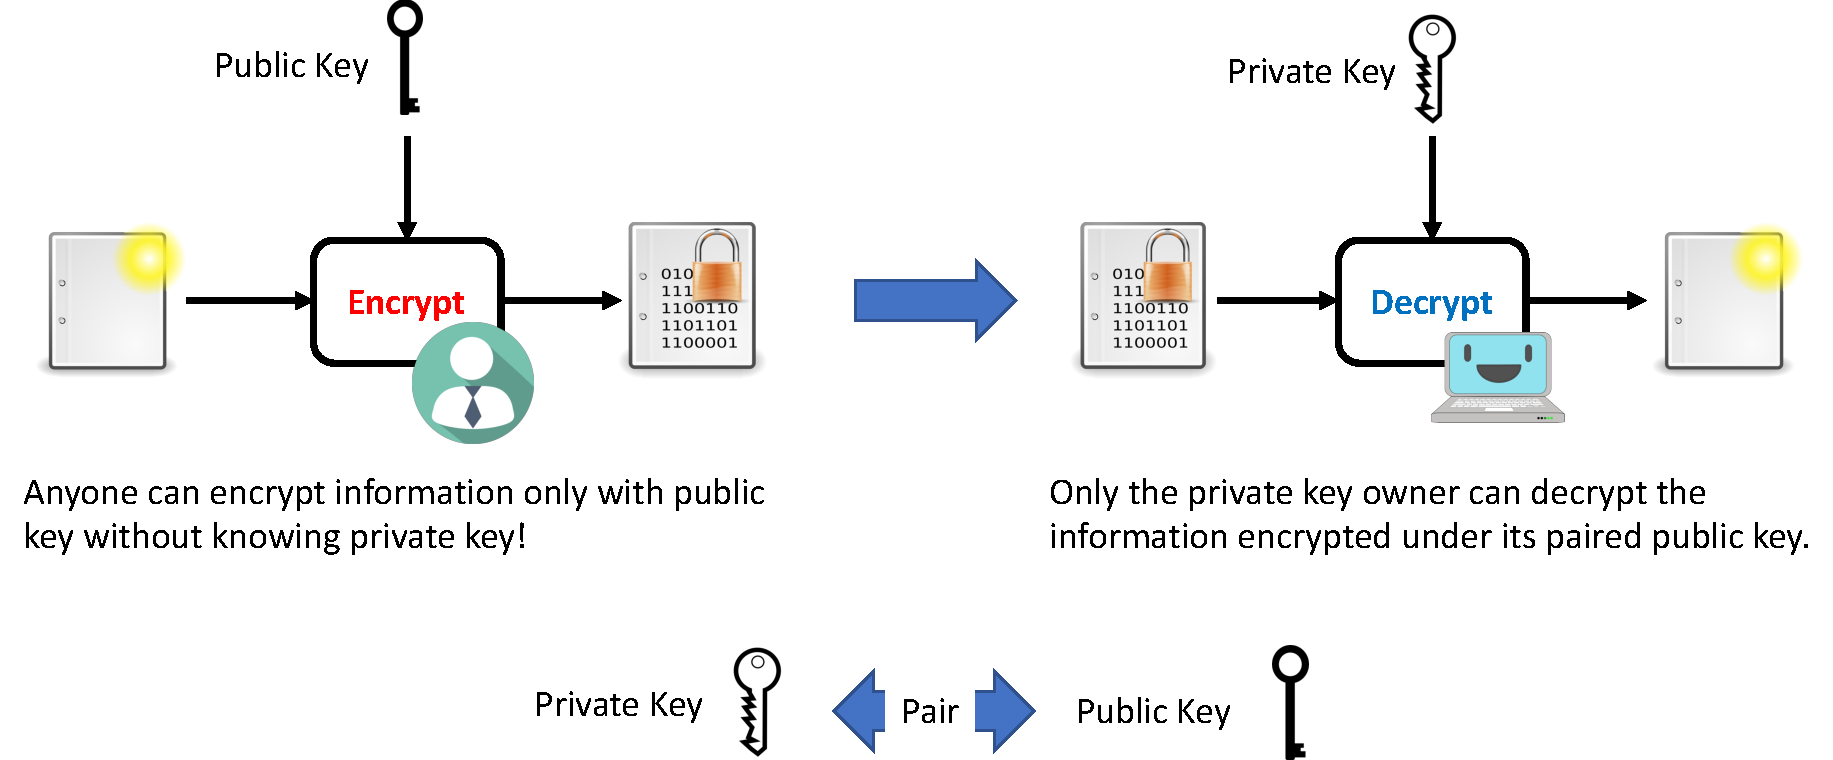
\includegraphics[width=\linewidth]{Figs/pk_cryptosystem.pdf}
\end{center}

\vspace{1ex}

$\Rightarrow$ AESなどにはない、非常に強力な暗号化の概念。現代のセキュリティインフラはこれで成り立っていると言っても過言ではない。
\end{frame}

\begin{frame}
今回は\underline{正しく・安全に}公開鍵暗号を使っていくためのお話。

\begin{block}{\small この講義で最終的に学びたいこと}
\begin{itemize}
\item 公開鍵暗号はどういうものか。AESと比べたpros/cons。
\item RSA暗号と楕円曲線暗号\footnote[frame]{楕円曲線Diffie-Hellmanを取り上げる}の違い。
\item AESと公開鍵暗号を組み合わせてデータを暗号化するために。
\end{itemize}
\end{block}

細かい話もするが、数式は使わない。

「イメージ」と「コードの流れ&その流れの必要性」をつかめるようにする。
\end{frame}


\begin{frame}
\frametitle{この講義の対象と事前準備}
対象:
\begin{itemize}
\item 暗号・セキュリティ技術に興味がある初学者
\item Webに暗号技術を導入したいWeb系のエンジニア
\end{itemize}

\vspace{2ex}

必須ではないが触って楽しむのには必要な事前準備:
\begin{itemize}
\item Bash, Gitが使えるようになっていること
\item Node.js, npm, yarnが使えるようになっていること
\item Google Chrome系ブラウザ and/or Firefoxが利用可能なこと
\end{itemize}
\end{frame}

\begin{frame}
今後の予定(暫定)
\begin{enumerate}
 \item \textcolor{gray}{導入\&JSの暗号化コードを触ってみる}
 \item \textcolor{gray}{AESを正しく・安全に暗号化するには?}
 \item \alert{公開鍵暗号はどうやって使う?その使い方のコツは?} ← 今日はココ
 \item ハッシュ・MAC・署名、それぞれの使い所と使い方は?
\end{enumerate}
「こういうのを知りたい」というリクエストがあれば是非。

\end{frame}

\begin{frame}
\frametitle{発表者紹介}
{\Large 栗原 淳 (Jun Kurihara)}
\begin{itemize}
 \item (株)ゼタント 主任研究員\\
(株) 国際電気通信基礎技術研究所(ATR) 連携研究員
 \item 博士(工学), \\
 専門: セキュリティ、応用数学、システムアーキテクチャとか
 \item  Webシステム(フロントエンド・バックエンド)を作ったり、論文他のアルゴリズムを実装したり、研究して論文書いたり、セキュリティ技術中心に手広くやってます。
 \item GitHub: \url{https://github.com/junkurihara}\\
LinkedIn: \url{https://www.linkedin.com/in/junkurihara}
\end{itemize}
\end{frame}
%%%%%%%%%%%%%%%%%%%%%%%%%%%%%%%%%%%%%%%%%%%%%%%%%%%%%%%%%%%%%%%%%%%%%%%%%%%%%%%%%%%%%%%%%%%%%%%%%%%
\section{公開鍵暗号の使い方 事始め}
\begin{frame}
\centering
{\Large 公開鍵暗号の使い方 事始め}
\end{frame}

\begin{frame}
\frametitle{公開鍵暗号の種類}
\begin{exampleblock}{}
\begin{center}
公開鍵暗号の定義「\underline{特殊な数学的条件}を満たす鍵ペアを生成」\\[0.5ex]
 $\Downarrow$\\[0.5ex]
この「数学的条件」に複数の種類が存在。
\end{center}
\end{exampleblock}

\vspace{2ex}

JavaScriptに限らず、各種環境で利用可能な代表的な公開鍵暗号:
\begin{itemize}
 \item 素因数分解に関する条件\\ → \alert{RSA暗号}
 \item 楕円曲線上の離散対数に関する条件\\ → \alert{楕円曲線暗号(Elliptic Curve Cryptography)}\footnote[frame]{\scriptsize 今回は便宜上Elliptic Curve Diffie-Hellman; ECDHを楕円曲線暗号と呼んでいく。}
\end{itemize}
この2つの使い方、注意ポイントを今回は取り上げる。
\end{frame}

\begin{frame}
\frametitle{RSA暗号のさわり}
\begin{block}{RSA Cryptography}
言わずもがな、公開鍵暗号の代表的な手法
\begin{itemize}
 \item 1977年、Rivest-Shamir-Edelmanの3名により発明。2000年に特許期間満了(現在特許フリー)。暗号化以外に「署名」の手法への応用も有名。
 \item RFC 8017 (PKCS\#1 v2.2)、ANSI X9.31、IEEE 1363、CRYPTREC等、各所で標準に採用。
 \item 公開鍵長は1024--4096bitsが標準的に使われている。\footnote[frame]{原理的には無限に伸ばせる。}
 \item 暗号化・署名の際には、元のデータにパディングが必要。\alert{パディング方法によりセキュリティが大きく左右される。}\footnote[frame]{RSA-OAEP(暗号化)、RSA-PSS(署名)が現状ベターな方法。これを話す。}
\end{itemize}
\end{block}

\end{frame}

\begin{frame}
\frametitle{楕円曲線暗号のさわり}
\begin{block}{Elliptic-Curve Cryptography}
楕円曲線という数の世界での「離散対数」を使った方式の総称\footnote[frame]{\scriptsize 普通に離散対数問題を使うより、楕円曲線上でやることで安全性を担保する鍵長が短くなる。}
\begin{itemize}
\item 1985年頃、Victor Miller、Neal Koblitzにより独立に考案。
\item Diffie-Hellman(DH)\footnote[frame]{\scriptsize RFC2631 \url{https://tools.ietf.org/html/rfc2631}}を楕円曲線上で実行するのがECDH、DSA\footnote[frame]{\scriptsize NIST FIPS 186-4 \url{https://nvlpubs.nist.gov/nistpubs/FIPS/NIST.FIPS.186-4.pdf}}を楕円曲線上で実行するのがECDSA。
\item RFC8442、CRYPTREC、IEEE P1363等で標準化。TLSやBitcoinなど多方面で利用。
\item 公開鍵長は256--521bits (Compact form) が標準的に使われている。
\item ECDHは「ECDH-Ephemeral」という方法で実行することで、普通に使うより\alert{安全性が大きく向上}する。\footnote[frame]{\scriptsize Forward Secrecy(後述)を担保する。}
\end{itemize}
\end{block}
\end{frame}

\begin{frame}
\frametitle{AESと比べた公開鍵暗号のPros/Cons}
\small

何でもかんでも公開鍵暗号、で良さそうな気もしてくるが…

\begin{table}
\centering
\begin{tabular}{|p{0.1\linewidth}||p{0.39\linewidth}|p{0.39\linewidth}|}
\hline
 & \textbf{Pros} & \textbf{Cons}\\
\hline
\hline
\textbf{AES}
& ・安全性を担保する鍵長が短い (128bits〜) & ・パスワードなどの\structure{事前共有が必要} \\
& ・一般的に\alert{高速}・SoCでの最適化も望める\footnote[frame]{Intel AES-NI} & \\
\hline
\textbf{公開鍵暗号}
& ・パスワードなどの秘密情報の\alert{事前共有が不要} & ・安全性を担保する鍵長が長い (RSA: 2048bits〜)\\
& & ・一般的に\structure{非常に遅い・重い}\\
\hline
\end{tabular}
\end{table}

$\Rightarrow$ 使い所を考えて組み合わせて使う、もしくは場合に応じて使い分けないと\structure{実用に耐えないシステム・サービスが出来上がる}。


\end{frame}

\begin{frame}
\frametitle{安全性を担保する鍵長が大きく違うのはどういうこと?}

AESと比べたRSA・楕円曲線暗号の公開鍵のビット長比較\footnote[frame]{\scriptsize Recommendation for Key Management, Special Publication 800-57 Part 1 Rev. 4, NIST, 01/2016. \url{https://csrc.nist.gov/publications/detail/sp/800-57-part-1/rev-4/final}}。

\alert{横1行がだいたい同じくらいの安全性}と言われる。
\begin{table}
\centering
\begin{tabular}{|c||c|c|}
\hline
\textbf{AES} & \textbf{RSA} & \textbf{楕円曲線}\\
\hline
\hline
128 & 3072 & 256--383\\
\hline
192 & 7680 & 384--511\\
\hline
256 & 15360 & 512--\\
\hline
\end{tabular}
\end{table}

\begin{block}{}
AESに比べて、\alert{楕円曲線で倍、RSAに至っては24倍以上}の鍵長を使わないと、同じくらいの安全性を担保できない。
\end{block}

\structure{鍵長が長いほど、暗号化・復号がどんどん重く・遅くなっていく…}

\end{frame}
\begin{frame}
 
「AES-128が、RSA-3072と同じくらい」というイメージは、以下のように説明できる。
\begin{itemize}
 \item AES: 数値$=0,1,\dots,2^{128}-1$のうち、どれか1つが鍵。
 \item RSA: \alert{特殊な条件を満たす数 = 素数2個の積(合成数)}を選んで、公開・秘密鍵を求める。
\end{itemize}

\begin{center}
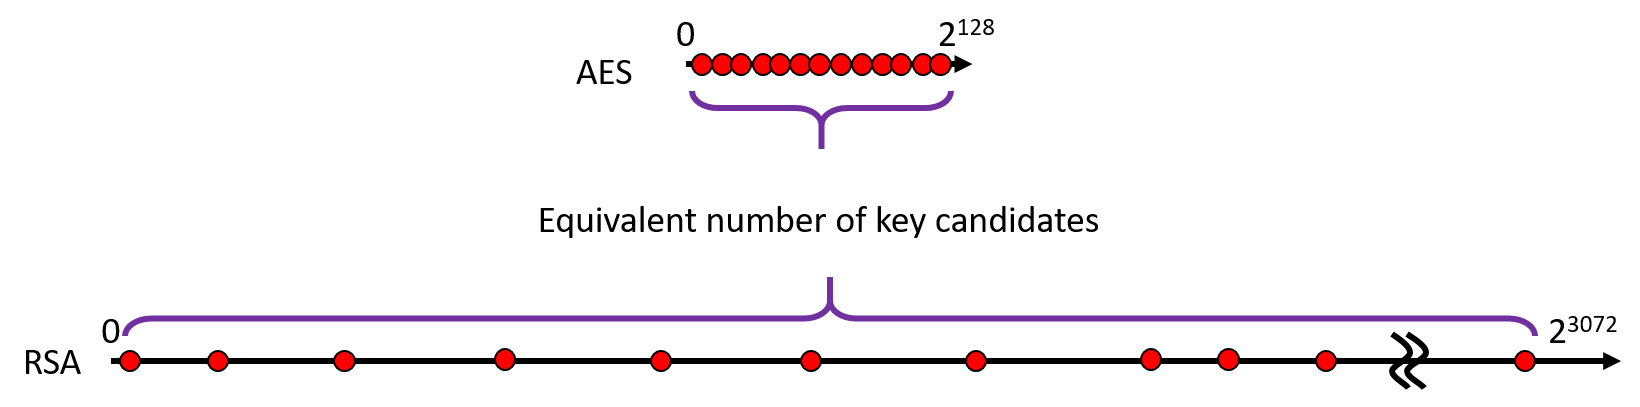
\includegraphics[width=\linewidth]{Figs/key-length-image.png} % todo
\end{center}

総当たりした時に\alert{「当たる」確率を揃えるには、RSAはその分巨大な数まで候補にしないとならない}。
\end{frame}

%%%%%%%%%%%%%%%%%%%%%%%%%%%%%%%%%%%%%%%%%%%%%%%%%%%%%%%%%%%%%%%%%%%%%%%%%%%%%%%%%%%%%%%%%%%%%%%%%%%
\section{今回のサンプル}
\begin{frame}
\centering
{\Large サンプルコードの準備}
\end{frame}

\begin{frame}
\frametitle{準備}
\small
細かく暗号化の説明を聞きつつ、手を動かすため、まず環境準備。

\alert{今回は、JavaScript (Node.js) を使って手元で公開鍵暗号化・復号。}

\begin{center}
 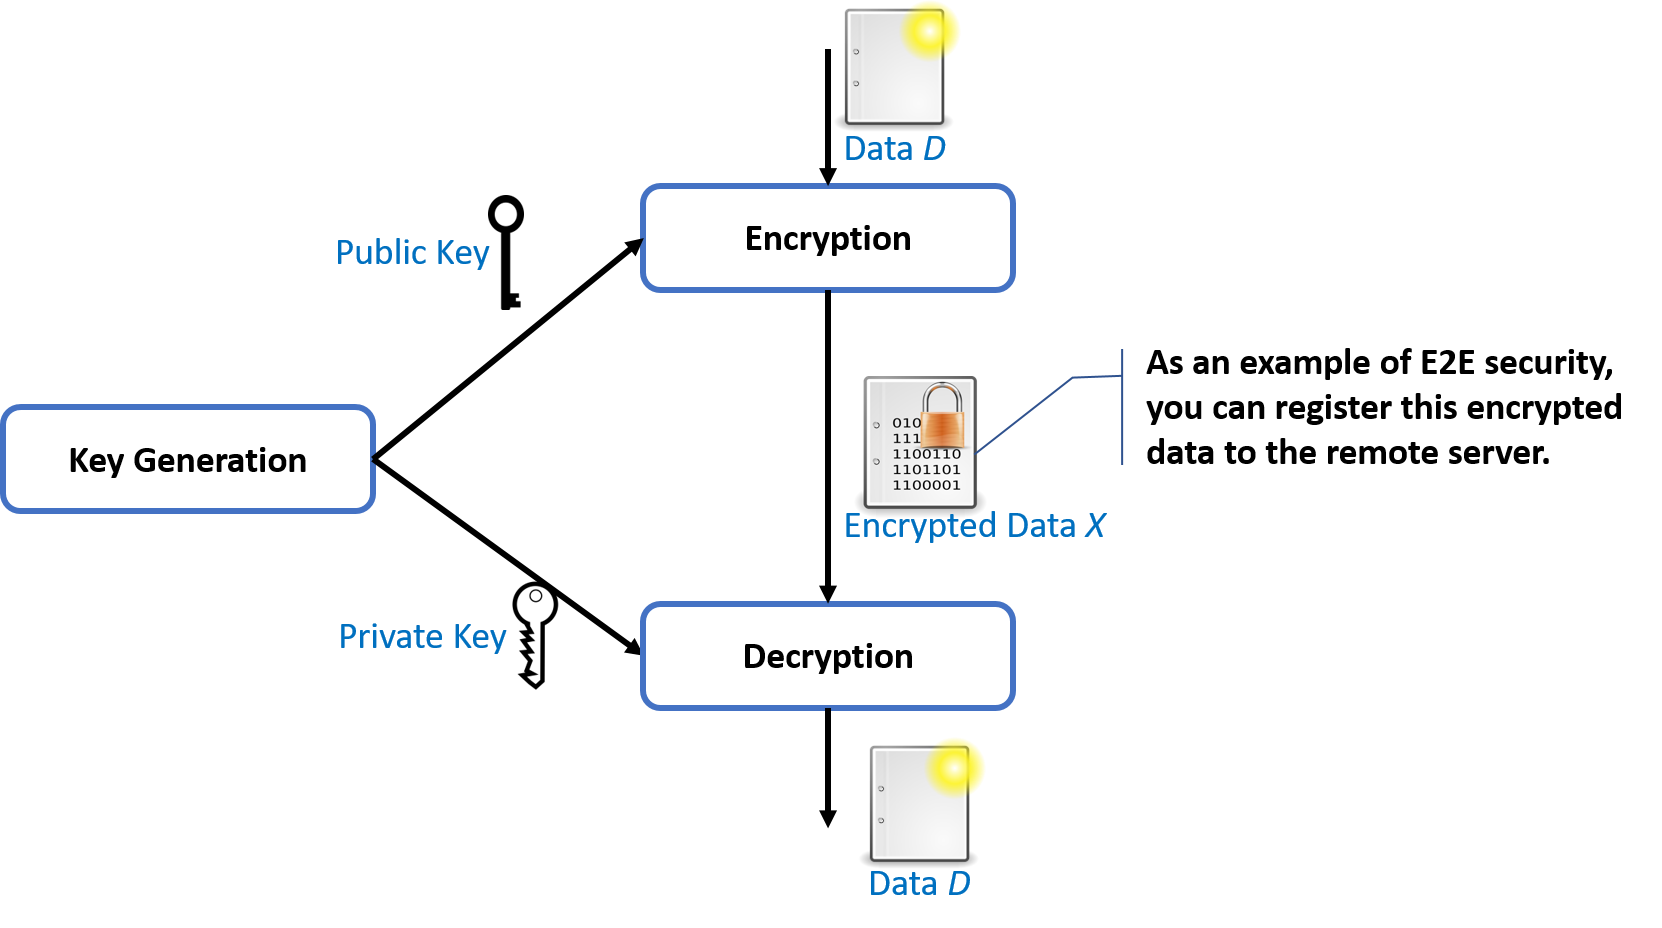
\includegraphics[width=0.8\linewidth]{Figs/pk-flow.png}%todo
\end{center}

\alert{サンプルコードはブラウザでも動く}。src/commands-browser.htmlを開くとこれからNode.JSで試すデモが開発者コンソールで実行される。適宜試したり比較すると良い。
\end{frame}

\begin{frame}
 
前回・前々回使った「リモートサーバに登録する」というところは、簡略化のため省略した。興味があれば、前回のコードを公開鍵暗号に拡張して、ネットワークを介してE2Eセキュリティしてみよう!
\end{frame}

\begin{frame}
\frametitle{環境}
以下の環境が前提:
\begin{itemize}
 \item Node.js ($>$ v10)がインストール済。yarnが使えること。 \footnote[frame]{インストールコマンド: \texttt{npm i -g yarn}}
 \item ブラウザとして、Google Chrome (系ブラウザ)、もしくはFirefoxがインストール済み
 \item Visual Studio Code や WebStorm などの統合開発環境がセットアップ済みだとなお良い。
\end{itemize}
\end{frame}

\begin{frame}
\frametitle{JavaScriptプロジェクトの準備}
\begin{itemize}
\item プロジェクトのGitHubリポジトリ\footnote[frame]{\url{https://github.com/zettant/e2e-security-03}}をClone\\
\begin{exampleblock}{}
\footnotesize
\$ \texttt{git clone https://github.com/zettant/e2e-security-03}\\
\$ \texttt{cd e2e-security-03/sample}
\end{exampleblock}
\item 依存パッケージのインストール
\begin{exampleblock}{}
\$ \texttt{yarn install}
\end{exampleblock}
\item ライブラリのビルド
\begin{exampleblock}{}
\$ \texttt{yarn build}
\end{exampleblock}
\end{itemize}
\end{frame}

%%%%%%%%%%%%%%%%%%%%%%%%%%%%%%%%%%%%%%%%%%%%%%%%%%%%%%%%%%%%%%%%%%%%%%%%%%%%%%%%%%%%%%%%%%%%%%%%%%%
\section{RSA暗号を使ってみよう}
\begin{frame}
\centering
{\Large RSA暗号を使ってみよう}
\end{frame}

\begin{frame}
\frametitle{RSA暗号を使うためのお作法}
\begin{block}{\small RSA暗号化の制限}
\alert{データ$D$と、公開鍵$PK$とが、同じビット長でなければならない}
\end{block}
$\Rightarrow$ RSA暗号化の前には、まず\underline{元データへのパディング}\footnote[frame]{\scriptsize 長いデータの場合は切断…}が必要。

\begin{center}
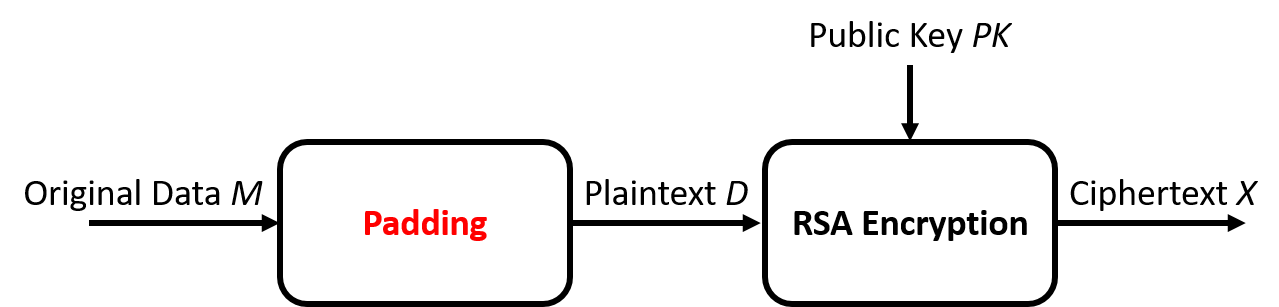
\includegraphics[width=0.9\linewidth]{Figs/rsa-padding.png}\\%todo
\end{center}
\vspace{2ex}

\alert{RSA暗号化には、前処理としてのパディングの選択が最重要のお作法。}
\end{frame}

\begin{frame}

RSA向けに主として2種類のパディング方法が知られている。\footnote[frame]{\scriptsize 共にPKCS\#1 (RFC8017) で標準化。\url{https://tools.ietf.org/html/rfc8017}}

\begin{itemize}
 \item PKCS\#1-v1.5 Padding
 \item Optimal Asymmetric Encryption Padding (OAEP)
\end{itemize}

\end{frame}


\begin{frame}

\begin{block}{\small PKCS\#1-v1.5 Padding}
\small
\begin{itemize}
 \item RSA暗号化と組み合わせると、RSAES-PKCS1-v1\_5。
 \item 元データ$M$に、公開鍵長まで以下のようなパディングを付与。
\begin{align*}
 D = \mathtt{0x00}\ ||\ \mathtt{0x02}\ ||\ \texttt{RandomSequence}\ ||\ \mathtt{0x00}\ ||\ M
\end{align*}
 \item 暗号化データを任意に改変でき、復号者に復号成功・失敗を確認させられる時、\alert{元データを復号される脆弱性}が知られている。\footnote[frame]{\scriptsize 1998年のBleinchenbacher's Attack。 2018年、現代のInternetでも未対策ホスト・サービスが大量なことが発表されている(ROBOT Attack)。}
 \item PKCS\#1 v2.2 (RFC8017) で「後方互換性のため以外では使用するな」と明示的に記載。CRYPTRECにおいても推奨暗号方式リストからドロップ。\footnote[frame]{\scriptsize \url{https://www.cryptrec.go.jp/method.html}}
\end{itemize}
\end{block}

\begin{center}
 {\Large \alert{基本的に使うな}}
\end{center}
\end{frame}

\begin{frame}

\begin{block}{\small Optimal Asymmetric Encryption Padding (OAEP) \footnote[frame]{\scriptsize M. Bellare and P. Rogaway, ``Optimal Asymmetric Encryption,'' in Proc. EUROCRYPTO 1994, pp.~92--111, LNCS 950, 1994.}}
\small
\begin{itemize}
 \item RSA暗号化と組み合わせて、RSA-OAEP、もしくはRSAES (RSA Encryption Scheme) - OAEPと呼ぶ。
 \item 元データ$M$とランダムシードに対して、All or Nothing Transform (AONT)を実行し、$D$を公開鍵ビット長まで膨らませる。
\begin{align*}
 D = \textsf{AONT}(M, \texttt{RandomSeed})
\end{align*}
 \item PKCS\#1-v1.5 Paddingの脆弱性は潰されている。実用の上ですぐに致命的な脆弱性は知られていない。PKCS\#1 v2.2 (RFC8017) では、\alert{新規アプリはOAEPを利用すること}と明記。
\end{itemize}
\end{block}

\begin{center}
 {\Large \alert{今はRSAならOAEP使っとけば間違いない}}
\end{center}
\end{frame}

\begin{frame}
\frametitle{参考: OAEPのイメージ図}
\begin{center}
 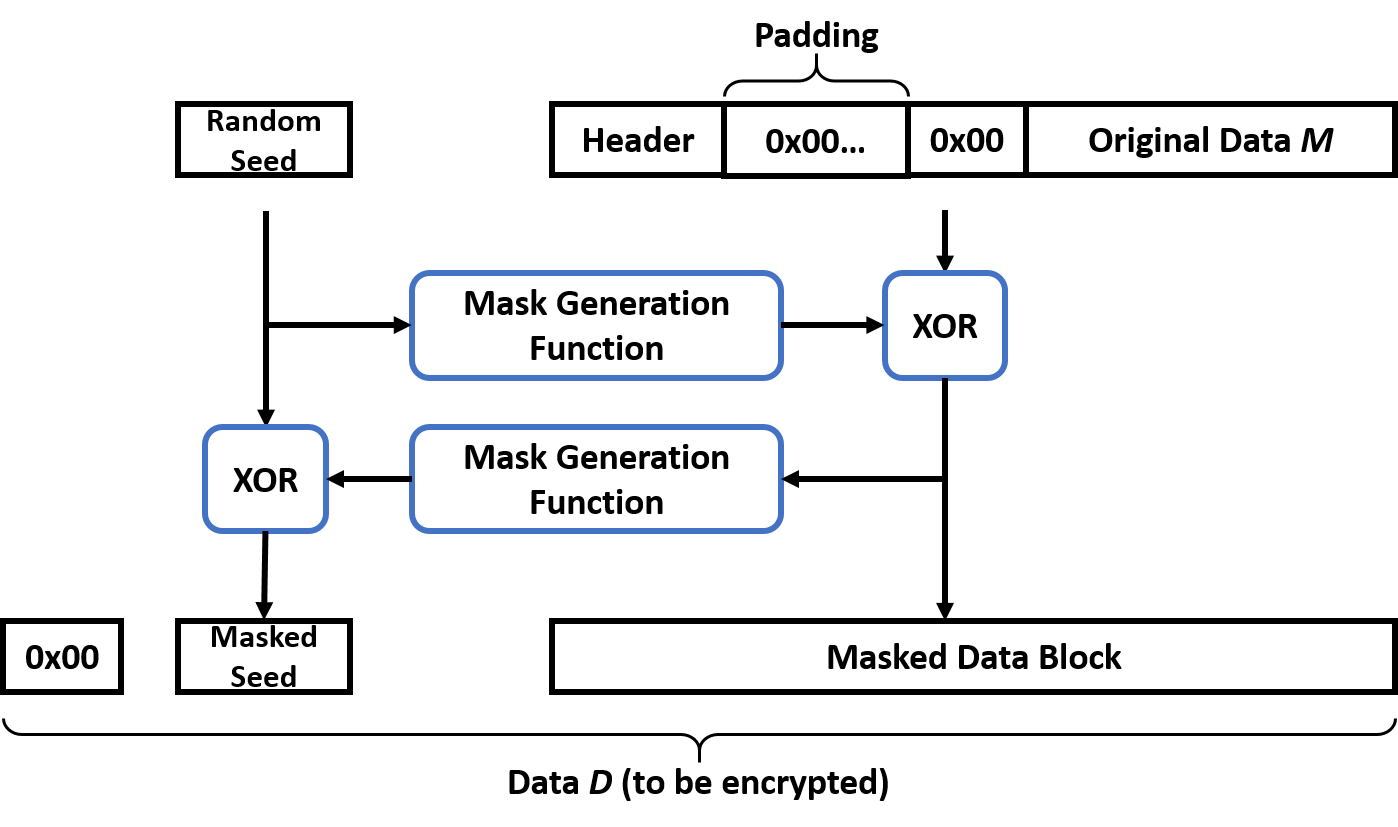
\includegraphics[width=\linewidth]{Figs/oaep.png}
\end{center}
逆変換はMasked Seed, Masked Data Blockが両方揃えば可能。
\end{frame}


\begin{frame}[fragile]
\frametitle{JavaScriptでRSA-OAEP暗号化をしてみよう}
sampleディレクトリで以下を実行すると、公開鍵・秘密鍵ペアを生成して、引数のstringの暗号化→復号を一連で実行する。
\begin{exampleblock}{}
\scriptsize
\begin{verbatim}
$ yarn execute rsa-oaep-demo 'hello world'
<Input Data>
hello world
<Generated RSA Key Pair (PEM Form)>
Public Key:
30820122300d06092a864....... // 生成した公開鍵(DER)
Private Key:
308204bc020100300d060....... // 生成した秘密鍵(DER)
=======

<Encrypted Data (in Base64)>
9f28a2acbd7cd5bc748f3....... // 'hello world'のRSA-OAEP暗号化データ
=======

<Decrypted Data>
hello world // 復号したデータ
=======
\end{verbatim}
\end{exampleblock}
\end{frame}

\begin{frame}[fragile]
\small
一連の動作をオートでやらずに自力でやる方法 (コピペで頑張る):
\begin{exampleblock}{\small RSA鍵ペアを生成}
\scriptsize
\begin{verbatim}
$ yarn execute rsa-keygen
<Generated RSA Key Pair (DER Form)>
Public Key:
30820122300d06092a864886f70d010......
Private Key:
308204be020100300d06092a864886f......
\end{verbatim}
\end{exampleblock}
\begin{exampleblock}{\small RSA-OAEP暗号化 (-pで公開鍵を指定)}
\scriptsize
\begin{verbatim}
$ yarn execute rsa-oaep-encrypt 'hello world'\
 -p '308201223......'
<Encrypted Data (in HexString)>
8da122191b1ec6da72afe88c96cfbb3...... // 暗号化データ
\end{verbatim}
\end{exampleblock}
\begin{exampleblock}{\small RSA-OAEP復号 (-sで秘密鍵を指定)}
\scriptsize
\begin{verbatim}
$ yarn execute rsa-oaep-decrypt '8da122191b1ec6da72afe88c96cfbb3......'\
 -s '308204be020100300d06092a864886f......'
<Decrypted Data>
hello world
\end{verbatim}
\end{exampleblock}
\end{frame}


\begin{frame}[fragile]
RSA-OAEPによる公開鍵暗号化のコードはこんな感じ。
\begin{block}{\small RSA鍵ペア生成 (src/test-api.js)}
\scriptsize
\begin{verbatim}
// bits = 2048
const jscu = getJscu(); // jscuオブジェクト取得。Node.js Crypto, WebCryptoのラッパー
const keyPair = await jscu.pkc.generateKey(
  'RSA', 
  {modulusLength: bits} // 2048bitsのRSA鍵ペアを生成
); 
\end{verbatim}
\end{block}
\begin{block}{\small RSA-OAEP暗号化 (src/test-api.js)}
\scriptsize
\begin{verbatim}
const jscu = getJscu(); // jscuオブジェクト取得。Node.js Crypto, WebCryptoのラッパー

// DERエンコード(Uint8Array)の公開鍵をjscuの鍵オブジェクトに変換。
const publicKey = new jscu.Key('der', publicDer);

const encrypted = await jscu.pkc.encrypt(
  uint8ArrayData, // 暗号化されるデータ
  publicKey,
  {hash: 'SHA-256'} // OAEPで利用されるハッシュ。今なら'SHA-256'使っとけばいい。
);
\end{verbatim}
\end{block}
\end{frame}
\begin{frame}[fragile]
\begin{block}{\small RSA-OAEP復号 (src/test-api.js)}
\scriptsize
\begin{verbatim}
const jscu = getJscu(); // jscuオブジェクト取得。Node.js Crypto, WebCryptoのラッパー

// DERエンコード(Uint8Array)の秘密鍵をjscuの鍵オブジェクトに変換。
const privateKey = new jscu.Key('der', privateDer);

const decrypted = await jscu.pkc.decrypt(
  uint8ArrayEncryptedData,
  privateKey,
  {hash: 'SHA-256'} // 暗号化で使われているものと一緒。
);
\end{verbatim}
\end{block}
これらのコードはjscuを使う限りはNode.jsでもブラウザでも一緒。
\end{frame}

\begin{frame}
RSAES-OAEPは、WebCrypto API(ブラウザ)でも、Node.js Cryptoでもネイティブサポートされている。\footnote[frame]{\scriptsize WebCryptoでは、「サポートされているブラウザだといいですね」。jscuだとその辺はpurejsで実装し直しているので動かないことはない。(IEはダメかも)}

\vspace{1ex}

なお、RSAES-PKCS1-v1\_5も規格上サポートされている。JSに限らず、\underline{どちらかというとOAEPの方がまだ実装されていない。}

\vspace{1ex}

$\Rightarrow $そのせいで、SSL/TLSではROBOT攻撃に対する脆弱性とかを引き起こしている……
\end{frame}



%%%%%%%%%%%%%%%%%%%%%%%%%%%%%%%%%%%%%%%%%%%%%%%%%%%%%%%%%%%%%%%%%%%%%%%%%%%%%%%%%%%%%%%%%%%%%%%%%%%
\section{楕円曲線暗号(ECDH)を使ってみよう}
\begin{frame}
\centering
{\Large 楕円曲線暗号(ECDH)を使ってみよう}
\end{frame}

\begin{frame}
\frametitle{楕円曲線暗号を使うためのお作法 その1}

今までECDHを公開鍵暗号って呼んでいてすみませんでした…

\begin{block}{\small Elliptic-Curve Diffie-Hellman (ECDH)}
ECDH自身は、データの暗号化ではなく、公開鍵・秘密鍵を使って\alert{送受信者間で秘密裏にランダムビット列を共有するための方法}。
\end{block}

$\Rightarrow$ 共有したランダムビット列を鍵(の種)として用いて、AESとかでデータを暗号化。

\begin{center}
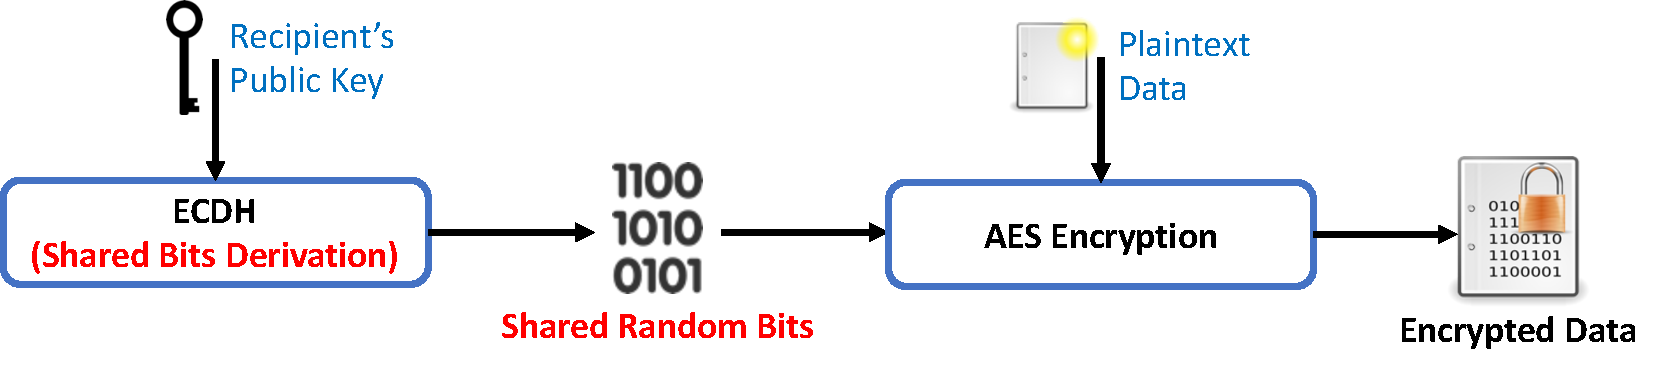
\includegraphics[width=\linewidth]{Figs/ecdh-flow01.pdf}

この流れ全体で「公開鍵暗号」の体を為す。
\end{center}

というわけで、まずはこの「共有ランダムビット列」の導出の話。
\end{frame}


\begin{frame}
(EC)DHにおける共有ランダムビット列の導出の流れ:
\begin{center}
 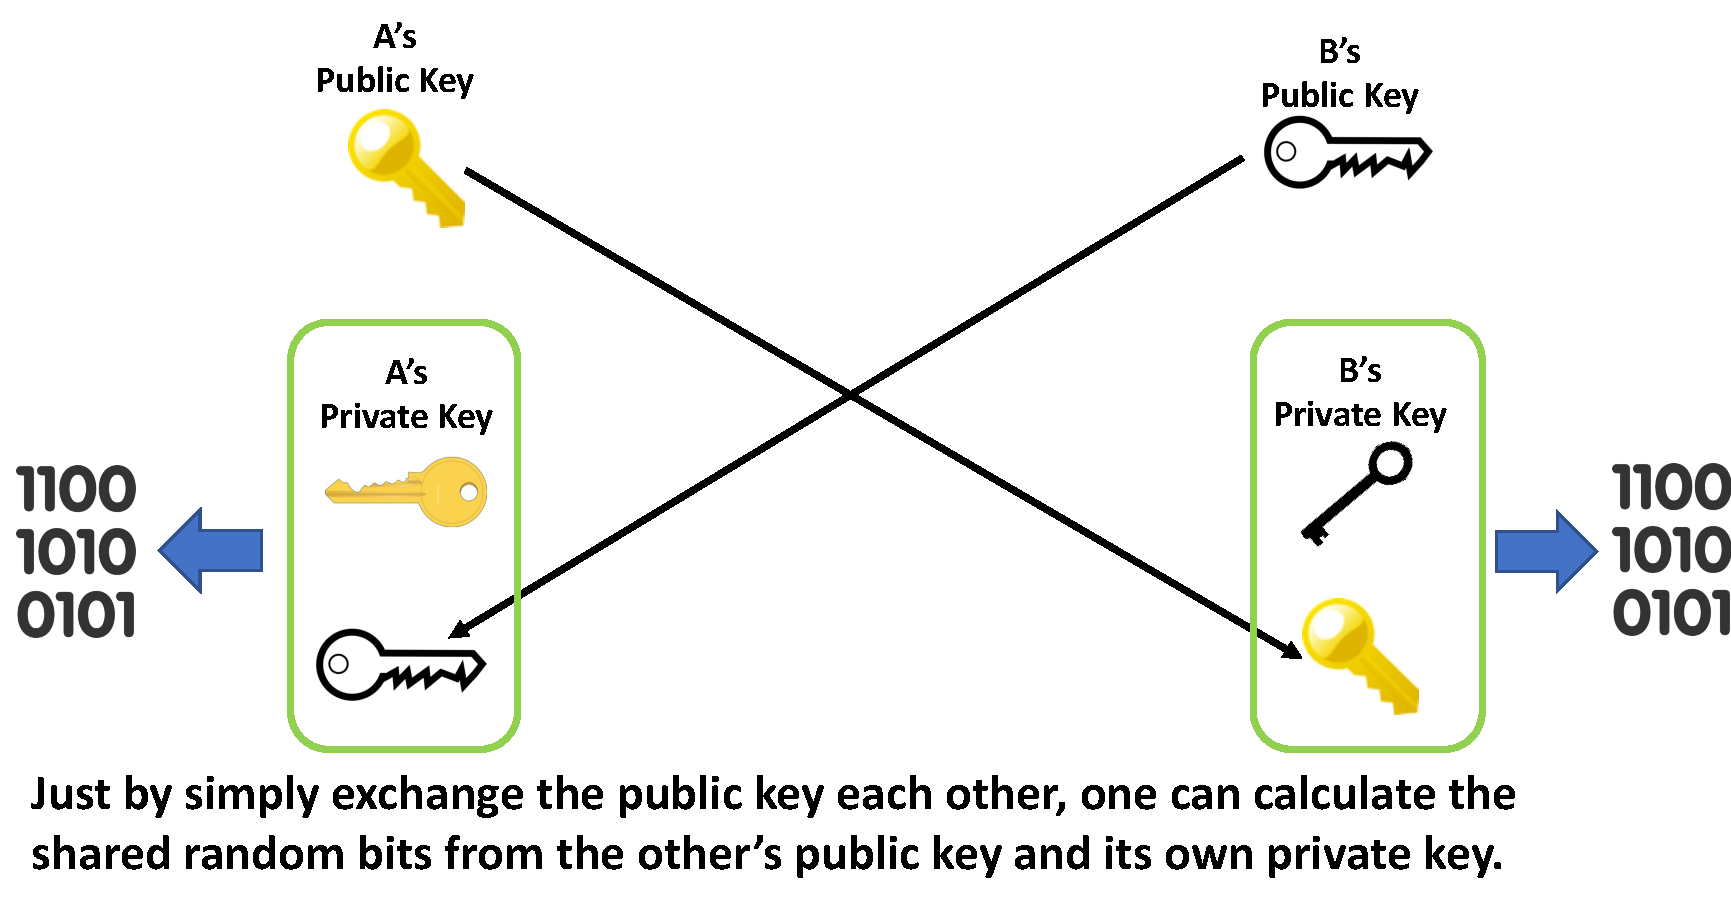
\includegraphics[width=\linewidth]{Figs/ecdh-flow02.pdf}
\end{center}
\vspace{-1ex}
送信者(A)と受信者(B)が、\alert{互いに公開鍵を交換するだけで同じビット列を秘密裏\footnote[frame]{\scriptsize 秘密鍵は一切表に出てこないことに注目}に共有}できる。
\end{frame}

\begin{frame}
ちょっとフォーマルに書くと:
\begin{block}{\small ECDHの特徴\footnote[frame]{\scriptsize ECでないDHも同様。}}
2つの公開鍵・秘密鍵ペア: \alert{$(\mathit{PK_1}, \mathit{SK}_1)$}と\textcolor{blue}{$(\mathit{PK_2}, \mathit{SK}_2)$}で、
\begin{align*}
\mathtt{SharedRandomBits} &= \mathsf{ECDH}(
\text{\textcolor{red}{$\mathit{PK}_1$}},
\text{\textcolor{blue}{$\mathit{SK}_2$}}
)\\
& = \mathsf{ECDH}(
\text{\textcolor{blue}{$\mathit{PK}_2$}},
\text{\textcolor{red}{$\mathit{SK}_1$}}
).
\end{align*}
すなわちECDHでは、\alert{鍵ペアを持っているもの同士なら、相手の公開鍵から共有ビット列が導出可能}。
\end{block}

共有ビット列の長さは、公開鍵長 (Compact form) と一緒。
\end{frame}

\begin{frame}[fragile]
\frametitle{JavaScriptでECDH共有ビット列導出をしてみよう}
sampleディレクトリで以下を実行。鍵ペアを2つ生成→互いの公開鍵から共有ビット列を生成する。

\begin{exampleblock}{}
\scriptsize
\begin{verbatim}
$ yarn execute check-ecdh
<ECC Key Pair A (DER Form)>
Public Key:
3059301306072a8648ce3d020106082... // 公開鍵A
Private Key:
308193020100301306072a8648ce3d0... // 秘密鍵A
=======
<ECC Key Pair B (DER Form)>
Public Key:
3059301306072a8648ce3d020106082... // 公開鍵B
Private Key:
308193020100301306072a8648ce3d0... // 秘密鍵B
=======

// 公開鍵Aと秘密鍵Bから生成
Shared Bits from Public Key A and Private Key B: c55393fc681811141...
// 公開鍵Bと秘密鍵Aから生成
Shared Bits from Public Key B and Private Key A: c55393fc681811141...
\end{verbatim}
\end{exampleblock}
共有ビット列は全く同じものになっていることに注目
\end{frame}

\begin{frame}[fragile]
\small
ECDH共有ビット列導出のコードの中身はこんな感じ。
\begin{block}{\small src/test-api.js}
\scriptsize
\begin{verbatim}
const jscu = getJscu();
const jscec = getJscec(); //js-crypto-ecオブジェクト。jscuのサブモジュール。

// DERエンコードからjscu鍵オブジェクトを生成、そのあとJWKエンコードの鍵として出力
const publicKey = new jscu.Key('der', publicDer);
const privateKey = new jscu.Key('der', privateDer);
const publicJwk = await publicKey.export('jwk');
const privateJwk = await privateKey.export('jwk');

// 共有ビット列の出力
const derived = await jscec.deriveSecret(publicJwk, privateJwk);
\end{verbatim}
\end{block}
※jscuではECDH+AESという形式でAPIを提供しているため、ECDH自身は隠蔽している。
そのため、ECDHの仕組みをわかりやすくするためにサブモジュールを呼んでいる。
\end{frame}

\begin{frame}
ECDHの共有ビット列導出は、WebCrypto API(ブラウザ)でも、Node.js Cryptoでもネイティブサポートされている。\footnote[frame]{\scriptsize [ブラウザ] encryptなどというわかりやすいAPIではなく、deriveBits(ビット導出)。[Node.js] ECDHオブジェクト生成。}
\end{frame}

\begin{frame}
\frametitle{楕円曲線暗号を使うためのお作法 その2}
前回の「AESを使うために」で学んだことの復習。

\begin{block}{\small 前回の復習}
マスターシークレット(=ECDH共有ビット列)を元にAES暗号化を行うためには、
\alert{マスターシークレットから作る鍵のランダム具合の向上、鍵の総当たりの困難化}を施すと良い。
\end{block}


$\Rightarrow$ 共有ビット列に対して鍵導出関数を利用することで担保する。
\begin{itemize}
 \item HKDF (RFC5869)
 \item Concat KDF (RFC8039)\footnote[frame]{\scriptsize JOSE向けに標準化された鍵導出関数 \url{https://tools.ietf.org/html/rfc8037}}
 \item etc....
\end{itemize}
今回はHKDFを使う。
\end{frame}

\begin{frame}
\frametitle{JavaScriptでECDHからAES暗号化してみよう}
ECDH, HDKF, AESを組み合わせて、「公開鍵暗号化」してみる。

\begin{center}
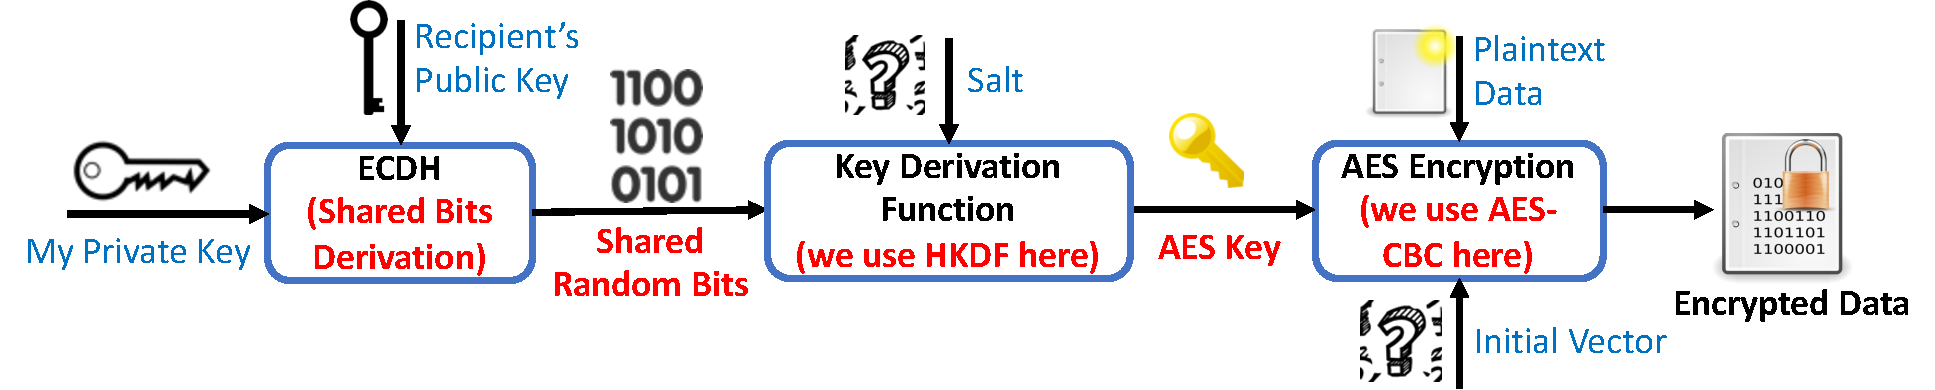
\includegraphics[width=\linewidth]{Figs/ecdh-flow03.pdf}
\end{center}

このフローでは、\alert{実際のデータの暗号化はAESに任せている}。
\begin{center}
 $\Downarrow$
\end{center}
RSA暗号化と違い、一度に暗号化できるデータサイズが公開鍵のサイズ以下などと制限されることはない。\footnote[frame]{\scriptsize ただし、通常この場合も共有ビット列を使って暗号化するデータは、「別のAES暗号化用の鍵(すなわち256bits以下)」とすることが多い。後述する。}
\end{frame}

\begin{frame}[fragile]
実行してみる。(コピペ頑張って!)

\begin{exampleblock}{\small EC鍵生成 (2回やって2ペア作る)}
\scriptsize
\begin{verbatim}
$ yarn execute ecc-keygen
<Generated ECC Key Pair (DER Form)>
Public Key:
3059301306072a8648ce3d020......
Private Key:
308193020100301306072a864.....

$ yarn execute ecc-keygen
<Generated ECC Key Pair (DER Form)>
Public Key:
3059301306072a8648ce3d020.....
Private Key:
308193020100301306072a864.....
\end{verbatim}
\end{exampleblock}
 
\end{frame}

\begin{frame}[fragile]
\begin{exampleblock}{\small ECDH+HKDF+AES-CBC暗号化}
\scriptsize
\begin{verbatim}
$ yarn execute ecdh-aes-encrypt 'hello world'\
-p '3059301306072a8648ce3d020106082a8648c......' // 送り先の公開鍵
-s '308193020100301306072a8648ce3d0201060......' // 送り元の秘密鍵

<Shared Bits> // ECDHの共有ビット列
51a1a502d01917e6ae0c7cd69cc7078d4a07d0172d271555d001485621551eef

<Derived AES Key> // HDKFで導出した鍵とパラメタ
Key: f52372329867b83ee4e2cada7452a909e85b1ffc2401c5e3b7e7aa7bf9363f7b
HKDF-Salt: 1dffbb6a9a0b91929b690116e3abd75b4a984e4d8686fcd9e35b4bd0220ebfe7
HKDF-Hash: SHA-256

<Encrypted data> // AES-CBC暗号化したデータ
Data: e36ded44e0e27a8f01d160feb54b1c30
Initial Vector: e9799bff5bdbd3400b1c753e5d5506ff

// Key, Salt, IV, Encrypted DataをMsgpackしたやつ
<Msgpacked encrypted and kdf data>
82a9656e6372797074656482a464617461d......
\end{verbatim}
\end{exampleblock}
パラメタがたくさんでコピペが無理なのでMsgpackでserializeして暗号化データを固めている。
\end{frame}

\begin{frame}[fragile]
\begin{exampleblock}{\small ECDH+HKDF+AES-CBC復号}
\scriptsize
\begin{verbatim}
// msgpackしたデータを秘密鍵にする。
$ yarn execute ecdh-aes-decrypt '82a9656e6372797074656482a46461......'
 -p '3059301306072a8648ce3d0201060......' // 送り元の公開鍵
 -s '308193020100301306072a8648ce3......' // 送り先の秘密鍵

<Shared Bits> // ECDHの共有ビット列
51a1a502d01917e6ae0c7cd69cc7078d4a07d0172d271555d001485621551eef

<Derived AES Key> // 共有ビット列とmsgpackの中のパラメタから導出した鍵
f52372329867b83ee4e2cada7452a909e85b1ffc2401c5e3b7e7aa7bf9363f7b

<Decrypted Data> // 復号データ
hello world
\end{verbatim}
\end{exampleblock}
\end{frame}


\begin{frame}[fragile]
ECDH, HKDF, AESを組み合わせた暗号化のコードはこんな感じ。
\begin{block}{\small 暗号化: src/commands-node.js}
\scriptsize
\begin{verbatim}
// Shared bits
const sharedBits = await ecdh(publicKeyA, privateKeyB);

// HKDF key derivation
const aesKey = await deriveKeyFromMasterSecret(sharedBits, 32);

// AES-CBC encryption
const encrypted = await encryptAES(data, aesKey.key);

// packing for ease
const packed = msgpack.encode({encrypted, kdfParams: aesKey.kdfParams});
\end{verbatim}
\end{block}
\end{frame}

\begin{frame}[fragile]
\begin{block}{\small 復号: src/commands-node.js}
\scriptsize
\begin{verbatim}
const depack = msgpack.decode(uint8ArrayData);

// Shared bits
const sharedBits = await ecdh(publicKeyB, privateKeyA);

// HKDF key derivation
const aesKey = await deriveKeyFromMasterSecret(
  sharedBits, 32, depack.kdfParams.salt, depack.kdfParams.hash
);

// AES-CBC decryption
const decrypted = await decryptAES(
  depack.encrypted.data, aesKey.key, depack.encrypted.iv
);
\end{verbatim}
\end{block}
\end{frame}


\section{より実用的な公開鍵暗号の運用}
\begin{frame}
\centering
{\Large より実用的な公開鍵暗号の運用}
\end{frame}

\begin{frame}
\frametitle{ここまでの振り返り}
ここ迄、以下の2つの「単純な」公開鍵暗号のやり方を学んだ。
\begin{itemize}
 \item RSA-OAEPによる暗号化
 \item ECDH, KDF, AESの組み合わせによる暗号化
\end{itemize}
\end{frame}

\begin{frame}
ただ、この単純なやり方だと、次のような制限がある。

\begin{itemize}
 \item 複数宛先向けの暗号化で\alert{めちゃくちゃ効率が悪い}。\\
 ※あるデータを、$n$人の宛先向けに暗号化すると、トータルの暗号化データは元のデータの$n$倍(以上)。
 \item \alert{秘密鍵$\mathit{SK}$が漏洩すると、何もかも終わり}。
\end{itemize}
\end{frame}

\begin{frame}
これを踏まえて、ここでそれらの実用的な対策を学ぶ。
\begin{enumerate}
\item \structure{公開鍵暗号によるAES暗号鍵のカプセル化}\\
$\Rightarrow$ 複数宛先向けに効率のいい公開鍵暗号化。
\item \structure{Perfect Forward Secrecy}\\
$\Rightarrow$ 秘密鍵が漏洩しても、過去の暗号化データはクラック不能。
\end{enumerate}
\end{frame}

\begin{frame}
\frametitle{公開鍵暗号による、AES暗号鍵のカプセル化}
\begin{block}{\small Hybrid Encryption, Key Encapsulation}
\begin{itemize}
 \item データの暗号化はランダム鍵$K$を使ったAES暗号化\footnote[frame]{\scriptsize 共通鍵暗号化}
 \item $K$のみを宛先ごとに公開鍵暗号化
\end{itemize}
\end{block}

\vspace{2ex}

\begin{center}
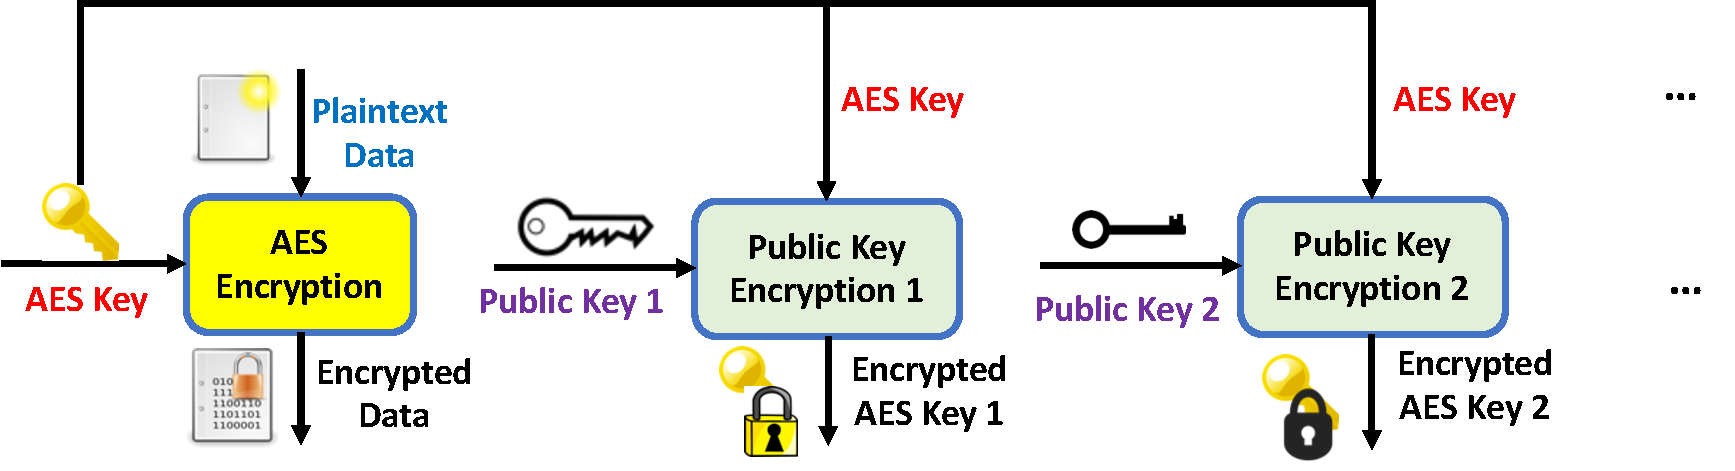
\includegraphics[width=\linewidth]{Figs/hybrid-encryption-flow01.pdf}
\end{center}
\end{frame}

\begin{frame}
\begin{itemize}
 \item 比較的小さいAESの鍵$K$のみ、宛先毎の公開鍵で暗号化。
 \item 鍵に比べて非常に大きい(であろう)\alert{データ部分の暗号化は、宛先に依らず共通化}してしまう。
\end{itemize}

\begin{block}{}
誰宛でもまず同じAES暗号化データを送りつけといて、そのAESの鍵だけを復号を許可したい人の公開鍵で暗号化するようなデータへのアクセス制御への応用。
\end{block}

\begin{block}{}
AES暗号化データ自体は誰宛でも共通なので、CDNに載せて公開配信とかしちゃうとめちゃくちゃ再利用性が高まってよい。\footnote[frame]{\scriptsize インターネット配信向けのDRMなんかでもこういう考え方がよく使われている。}
\end{block}

\end{frame}

\begin{frame}
\frametitle{Perfect Forward Secrecy}
より安全な暗号化のために。

\begin{block}{\small (Perfect) Forward Secrecy}
長期的に保存されているマスター秘密鍵の漏洩や、一部の暗号化データがクラックされたとしても、\alert{それ以外の過去に暗号化されたデータは復号されてしまうことはない}という概念。
\end{block}

\begin{center}
$\Downarrow$\\[1ex]

公開鍵・秘密鍵を1回限りで使い捨てる\alert{Ephemeral Scheme}の利用
\end{center}

\end{frame}

\begin{frame}
\begin{block}{\small なんでこんなめんどくさい概念が?}
「米国政府機関、SSL/TLSとかの暗号化通信データをそのままガンガン保存してる。保存しておいて、いつか復号できるような機会を待ってる。」とか暴露したことで注目を浴びている。
\end{block}
$\Rightarrow$ 保存データの一箇所でもクラックできたら、一気に他のデータもクラックできるのはよくない。\alert{被害は最小限にしよう}。
\end{frame}

\begin{frame}
 Ephemeral Schemeのイメージ

\begin{center}
 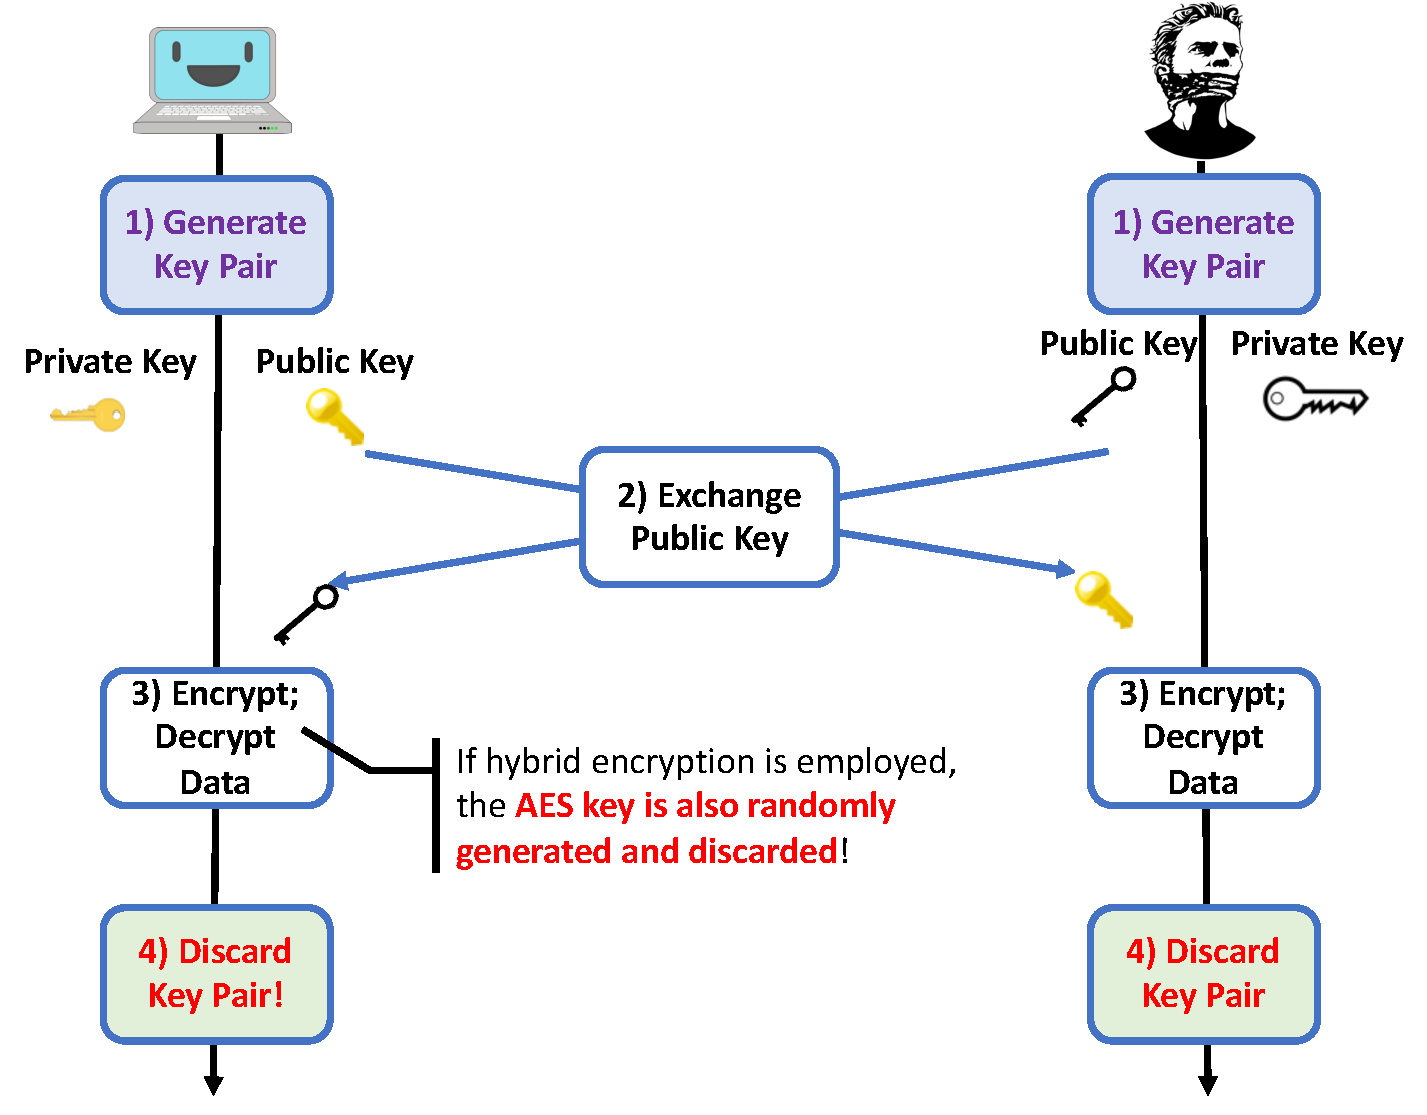
\includegraphics[width=0.8\linewidth]{Figs/ephemeral-scheme-flow01.pdf}
\end{center}
ハイブリッド暗号化の場合、\alert{AESの鍵自身もランダム\&使い捨て}
\end{frame}

\begin{frame}
ECDHを使った暗号化では、Ephemeral Schemeを使うのが推奨される\footnote[frame]{\scriptsize  RSA暗号を使った場合のEphemeral Schemeを標準の手法は知る限りない…単純に巨大な公開鍵を送るコストが高いことと、RSA-4096でAES-256の鍵を暗号化するなど、無駄の多さが理由か?}。


\begin{block}{\small ECDH-Ephemeral (ECDHE)\footnote[frame]{\scriptsize TLSで利用されるスキームだと思って良い \url{https://tools.ietf.org/html/rfc8422}}}
\begin{itemize}
 \item 送信先の相手を問わず、毎回違う共有ビット列が生成される。

$\Rightarrow$ 「今使った」共有ビット列や秘密鍵が盗まれても過去のデータは解読不能。i.e., \alert{Forward secrecy}。
 \item 毎度毎度、まずEphemeralな公開鍵を送らなければならず、\structure{通信コストは高い}。
 \item \structure{「送られてきたEphemeralな公開鍵は、本当に自分がやりとりしたい相手の公開鍵か?」を確認する手間}もかかる。
\end{itemize}
\end{block}

\end{frame}


\begin{frame}
\begin{block}{}
「送られてきたEphemeralな公開鍵は、本当に自分がやりとりしたい相手の公開鍵か?」を確認する手間もかかる。
\end{block}
\begin{center}
 $\Downarrow$\\
ここでようやく\\
\alert{本人確認・改ざん防止を担保をする「署名」を使う}。\\
次回の勉強会で話す予定。
\end{center}

\end{frame}

%%%%%%%%%%%%%%%%%%%%%%%%%%%%%%%%%%%%%%%%%%%%%%%%%%%%%%%%%%%%%%%%%%%%%%%%%%%%%%%%%%%%%%%%%%%%%%%%%%%
\section{まとめ}
\begin{frame}
 \centering
 {\Large まとめ}
\end{frame}

\begin{frame}
\frametitle{まとめ}
お疲れ様でした。

\begin{itemize}
\item 公開鍵暗号化の際のお作法を学んだ。
\begin{itemize}
 \item RSA: パディングには\alert{OAEPを使う(RSAES-OAEP)}。
 \item ECDH: 導出した共有ビット列は\alert{鍵導出関数を通してから}AESの鍵として利用する。
\end{itemize}
\item より実用的な公開鍵暗号化の運用について触れた。
\begin{itemize}
 \item \structure{ハイブリッド暗号化}: 複数人向け、量的に効率的な暗号化。
 \item \structure{Ephemeral Scheme}: Perfect Forward Secrecyを担保して万一の鍵漏洩に備える。
\end{itemize}
\item 上記について、JavaScriptのコードを実行/中身を覗いてみた。
\end{itemize}
\end{frame}


\begin{frame}
\frametitle{次回は}
内容: 
\begin{itemize}
 \item 暗号化に加えて、MAC・署名を使ってみよう(数学的なことはやらない)
 \item まずはハッシュ: SHA2, SHA3
 \item 共通鍵ベース: HMAC/CMAC
 \item 公開鍵ベース: RSA Signature/ECDSA
\end{itemize}

\end{frame}


\begin{frame}
\frametitle{宣伝: iTransfy by Zettant}
\begin{center}
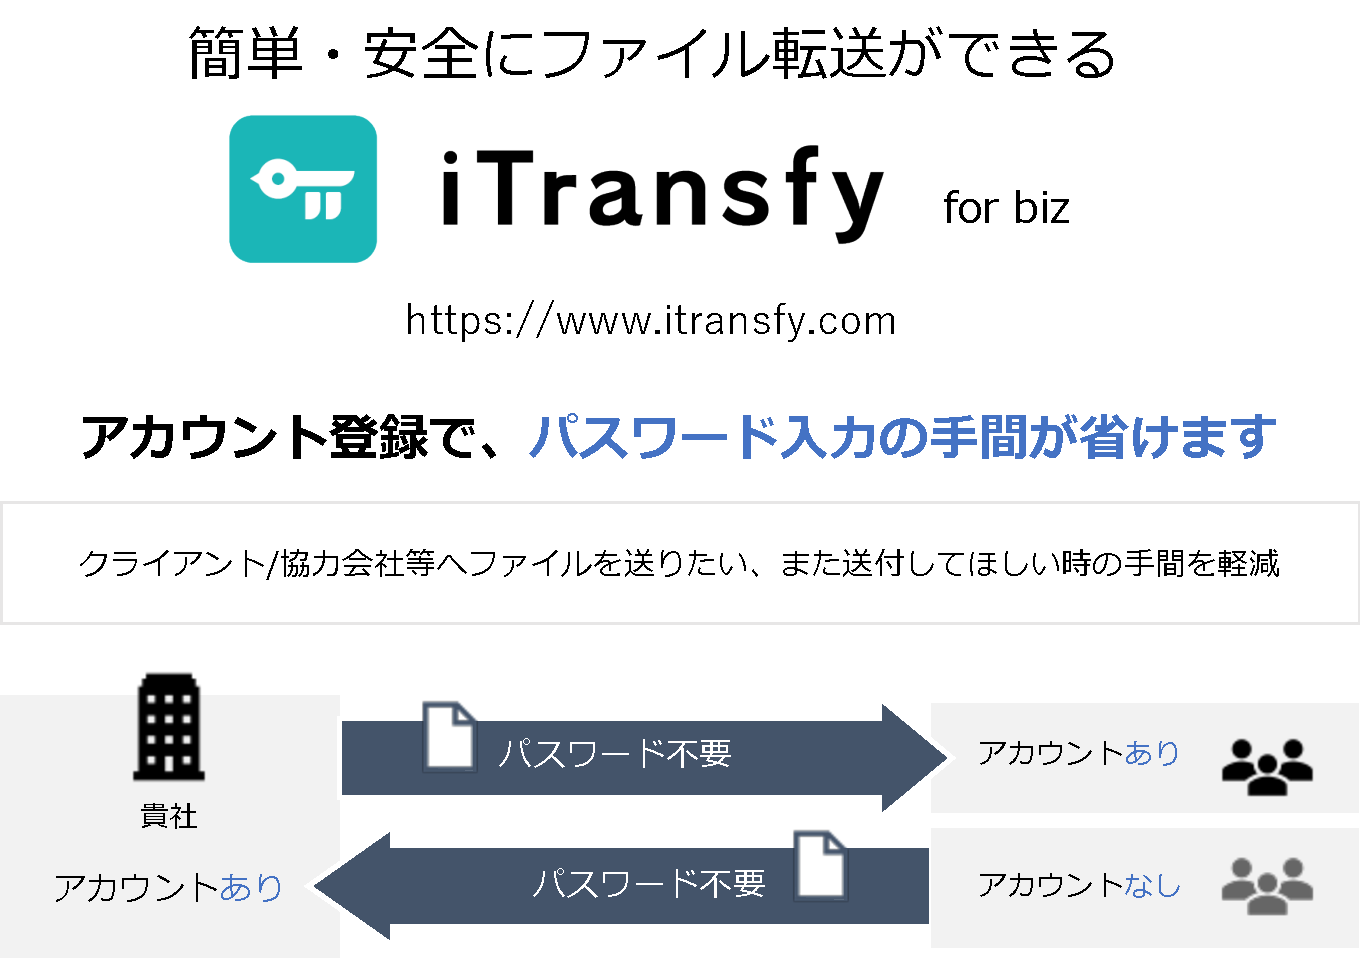
\includegraphics[width=0.9\linewidth]{FigsZettant/itransfy.pdf} 
\end{center}
\end{frame}

\begin{frame}
\frametitle{宣伝: 株式会社ゼタント}
\begin{tabular}{cc}
\begin{minipage}[b]{0.3\linewidth}

\includegraphics[width=\linewidth]{FigsZettant/logo.pdf}
\vspace{1ex}
\end{minipage}
 & 
\begin{minipage}[b]{0.7\linewidth}
\footnotesize
ゼタントはのミッションは、\\

「自分の身は自分で守ることができる世の中にする」\\

ことです。\\
共感してくれる仲間を募集しています!\\

問合せ先: \url{recruit@zettant.com}\\
会社URL: \url{https://www.zettant.com}
\end{minipage}
\end{tabular}
\end{frame}








% %%%%%%%%%%%%%%%%%%%%%%%%%%%%%%%%%%%%%%%%%%%%%%%%%%%%%%%%%%%%%%%%%%%%%%%%%%%%%%%%%%%%%%%%%%%%%%%%%%%
% \backupbegin

% \begin{frame}
%  以下バックアップ
% \end{frame}
% \begin{frame}
% 直接Concat KDFを暗号化の鍵にするか、
% あるいはConcat KDFの結果をAESKWの鍵としてContent Encryption Keyを暗号化するのに使う。

% \end{frame}

% \begin{frame}
% \frametitle{ECDH Ephemeral (ECDHE)}
% \begin{center}
% 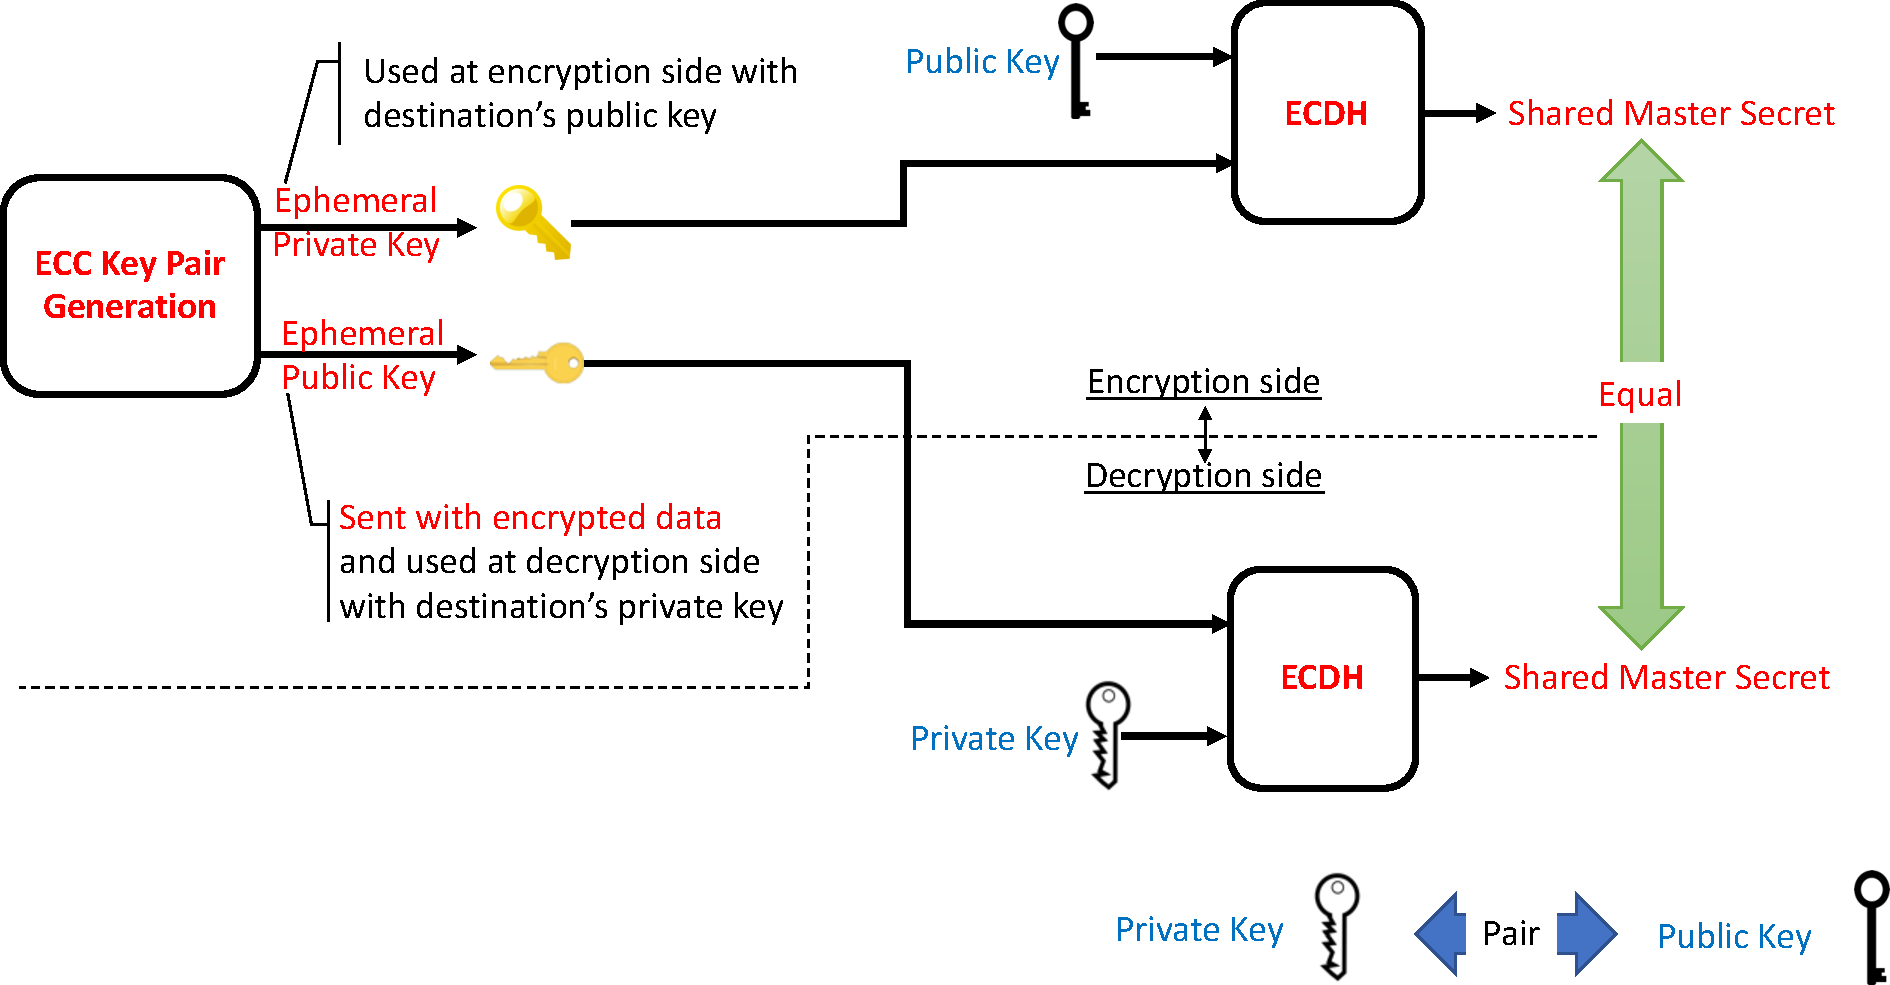
\includegraphics[width=\linewidth]{Figs/ecdh01.pdf}
% \end{center}
% \end{frame}

% \begin{frame}
% \begin{center}
% 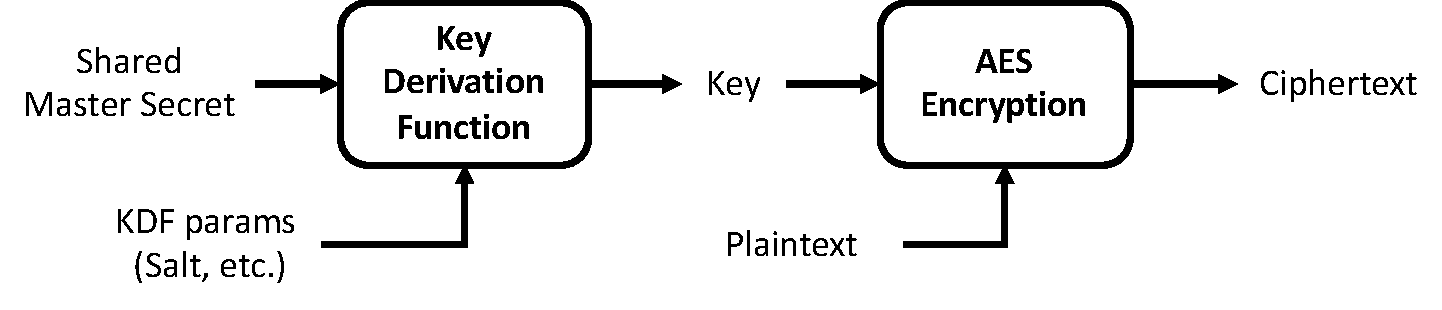
\includegraphics[width=\linewidth]{Figs/ecdh02.pdf}
% \end{center}
% \end{frame}


% \begin{frame}
% \begin{center}
% 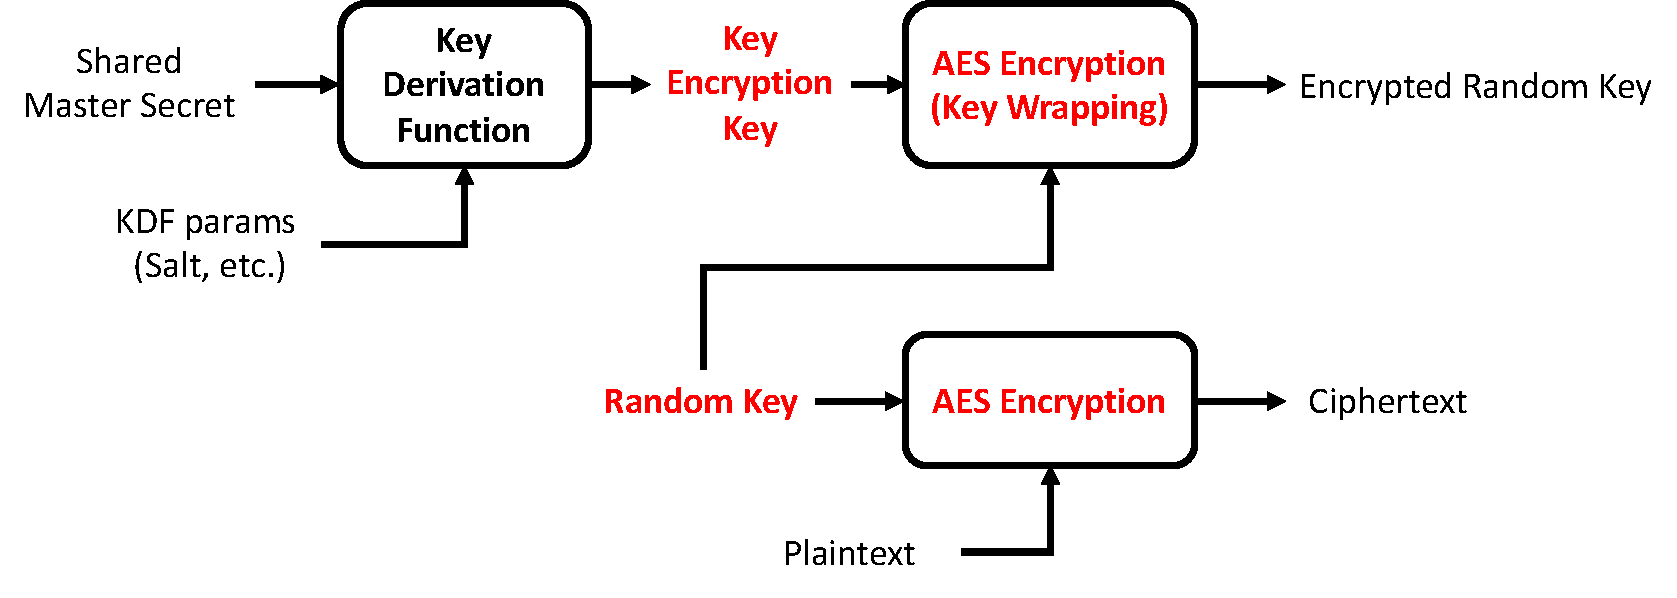
\includegraphics[width=\linewidth]{Figs/aeskw.pdf}
% \end{center}
% \end{frame}




% \section{Backup}

% \begin{frame}
 
% \end{frame}

% \begin{frame}
% \frametitle{Appendix}
% This page is not counted.
% \end{frame}
% \backupend
\end{document}
%%%%%%%%%%%%%%%%%%%%%%%%%%%%%%%%%%%%%%%%%%%%%%%%%%%%%%%%%%%%%%%%%%%%%%%%%%%%%%%%%%%%%%%%%%%%%%%%%%%
%%%%%%%%%%%%%%%%%%%%%%%%%%%%%%%%%%%%%%%%%%%%%%%%%%%%%%%%%%%%%%%%%%%%%%%%%%%%%%%%%%%%%%%%%%%%%%%%%%%
%%%%%%%%%%%%%%%%%%%%%%%%%%%%%%%%%%%%%%%%%%%%%%%%%%%%%%%%%%%%%%%%%%%%%%%%%%%%%%%%%%%%%%%%%%%%%%%%%%%
%%%%%%%%%%%%%%%%%%%%%%%%%%%%%%%%%%%%%%%%%%%%%%%%%%%%%%%%%%%%%%%%%%%%%%%%%%%%%%%%%%%%%%%%%%%%%%%%%%%
%%%%%%%%%%%%%%%%%%%%%%%%%%%%%%%%%%%%%%%%%%%%%%%%%%%%%%%%%%%%%%%%%%%%%%%%%%%%%%%%%%%%%%%%%%%%%%%%%%%
%%%%%%%%%%%%%%%%%%%%%%%%%%%%%%%%%%%%%%%%%%%%%%%%%%%%%%%%%%%%%%%%%%%%%%%%%%%%%%%%%%%%%%%%%%%%%%%%%%%
